%% To submit your paper:
%DIF LATEXDIFF DIFFERENCE FILE
%DIF DEL paper.tex      Sat Dec 31 11:12:30 2016
%DIF ADD paperMD2.tex   Sat Dec 31 11:12:06 2016
\documentclass[draft,linenumbers]{agujournal}
\draftfalse

%% For final version.
% \documentclass{agujournal}

\journalname{Water Resources Research}

\usepackage{url, bbm, comment}
%DIF PREAMBLE EXTENSION ADDED BY LATEXDIFF
%DIF UNDERLINE PREAMBLE %DIF PREAMBLE
\RequirePackage[normalem]{ulem} %DIF PREAMBLE
\RequirePackage{color}\definecolor{RED}{rgb}{1,0,0}\definecolor{BLUE}{rgb}{0,0,1} %DIF PREAMBLE
\providecommand{\DIFadd}[1]{{\protect\color{blue}\uwave{#1}}} %DIF PREAMBLE
\providecommand{\DIFdel}[1]{{\protect\color{red}\sout{#1}}}                      %DIF PREAMBLE
%DIF SAFE PREAMBLE %DIF PREAMBLE
\providecommand{\DIFaddbegin}{} %DIF PREAMBLE
\providecommand{\DIFaddend}{} %DIF PREAMBLE
\providecommand{\DIFdelbegin}{} %DIF PREAMBLE
\providecommand{\DIFdelend}{} %DIF PREAMBLE
%DIF FLOATSAFE PREAMBLE %DIF PREAMBLE
\providecommand{\DIFaddFL}[1]{\DIFadd{#1}} %DIF PREAMBLE
\providecommand{\DIFdelFL}[1]{\DIFdel{#1}} %DIF PREAMBLE
\providecommand{\DIFaddbeginFL}{} %DIF PREAMBLE
\providecommand{\DIFaddendFL}{} %DIF PREAMBLE
\providecommand{\DIFdelbeginFL}{} %DIF PREAMBLE
\providecommand{\DIFdelendFL}{} %DIF PREAMBLE
%DIF END PREAMBLE EXTENSION ADDED BY LATEXDIFF

\begin{document}


\title{I don't know, are you sure we want to do this?\\
Sea level adaptation decisions under uncertainty}

\authors{T. L. Thorarinsdottir\affil{1}, P. Guttorp\affil{1}, M. Drews\affil{2}, P. Skougaard Kaspersen\affil{2} and K. de Bruin\affil{3,4}}

\affiliation{1}{Norwegian Computing Center, Oslo, Norway}
\affiliation{2}{Technical University of Denmark, Copenhagen, Denmark}
\affiliation{3}{Center for International Climate and Environmental Research, Oslo, Norway}
\affiliation{4}{Wageningen Environmental Research, Wageningen, The Netherlands}

\correspondingauthor{T. L. Thorarinsdottir}{thordis@nr.no}

\begin{keypoints}
\item Decisions on adaptation measures need to take careful account of all uncertainties
\item Modeling local sea level rise is essential
\item Decisions under uncertainty do not have to be be based on precise costs
\end{keypoints}


\begin{abstract}
Sea level rise has serious consequences for harbor infrastructure, storm drains and sewer systems, and many other issues. Adapting to sea level rise requires comparing different possible adaptation strategies, comparing the cost of different actions (including no action), and assessing where and at what point in time the chosen strategy should be implemented. All these decisions must be made under considerable uncertainty--in the amount of sea level rise, in the cost and prioritization of adaptation actions, and in the implications of no action. Here we develop two illustrative examples: for Bergen on Norway's west coast and for Esbjerg on the west coast of Denmark, to highlight how technical efforts to understand and quantify uncertainties in hydrologic projections can be coupled with concrete decision-problems framed by the needs of the end-users using statistical formulations. Different components of uncertainty are visualized. We \DIFdelbegin \DIFdel{demonstrate }\DIFdelend \DIFaddbegin \DIFadd{demonstate }\DIFaddend the value of uncertainties and show for example that failing to take uncertainty into account can  result in the median projected damage costs being an order of magnitude smaller. 
\end{abstract}


%% ------------------------------------------------------------------------ %%
%  BEGIN ARTICLE
%% ------------------------------------------------------------------------ %%


\section{Introduction}\label{sec:intro}
The potential impact of climate change on local sea level, yielding effects such as frequent flooding, inundation and backflow of storm drainage and sewer systems, destructive erosion and contamination of wetlands and other habitats, requires city planners to make decisions in the presence of substantial uncertainty.

As adaptation decision-making is an ongoing process of weighing and choosing which measures should be taken at which moment in time \citep{Hallegatte&2012}, adaptive planning methods need to support decisions in the short term, while considering long-term developments. Challenges of adaptation decision-making under uncertainty relate to the incorporation of spatial, inter-temporal and flexibility aspects of adaptation priorities \citep{FankhauserSoare2013}, and the linkage with specific characteristics of sectors and contexts \citep{BisaroSwartHinkel2016, HinkelBisaro2016}. Several economic decision support tools and methods exist for adaptation assessment under uncertainty \citep[e.g.][]{Chambwera&2014, WilbyDessai2010, WalkerHaasnootKwakkel2013}. However, \citet{Watkiss&2015} conclude that these tools are very resource intensive and complex in the context of long-term adaptation investment decisions and call for the development of ``light touch'' approaches to better support local adaptation making.

In this paper we employ light touch decision tools to demonstrate the importance of combining projections of sea level rise and flood damages alongside a detailed quantification of both hydrologic and economic uncertainties in the context of real-life decision-problems experienced by stakeholders and authorities in two northern European cities, Bergen in Norway and Esbjerg in Denmark, see Figure~\ref{fig:CityMaps}. Based on communications with local end-users we highlight the value of taking into account uncertainty through two simplified and complementary case studies, where in the first one  planners want to know how early they should implement costly adaptation measures, whereas in the second case the aim is to highlight the risk of flooding in coastal areas, e.g. in order to prioritize future adaptation actions and investments. In both cases we show that embracing the uncertainties derived from economic and hydrologic models is absolutely crucial in order to answer the question of ``are we sure we want to do this?''

\begin{figure}[!hbpt]
\begin{center}
  \includegraphics[width=0.45\linewidth]{BergenMap.png}
  \includegraphics[width=0.45\linewidth]{EsbjergMap.png}
\caption{Terrain maps of central Bergen, Norway (left) and Esbjerg, Denmark (right).}
\label{fig:CityMaps}
\end{center}
\end{figure}

The Norwegian city of Bergen is the capital of Hordaland County. The city center is located on Byfjorden, and is surrounded by mountains. It has the largest port in Norway, both in terms of freight and passengers. The historic harbor area, Bryggen, is the only Hanseatic trade center remaining in its original style, and has been declared a UNESCO World Heritage site\footnote{See \url{http://whc.unesco.org/en/list/59}.}. Bryggen is regularly flooded at extreme tides, and it is feared that as sea levels rise, floods will become a major problem in other parts of Bergen as well \citep{bergenreport}.

The municipality of Bergen has, in cooperation with private actors, analyzed several possible adaptation measures against sea level rise. The measures range from an outer barrier that would protect the entire metropolitan area to various protection measures of limited areas in the inner harbor \citep{bergenreport}. While the viability of the constructions and the associated construction costs have been carefully analyzed, the optimal timing of potential adaptation measures and the effects of the associated uncertainties have yet to be investigated. We perform such an analysis where we consider uncertainty in projected sea level rise, damage costs, and the effect of sea level rise on changes in damage costs. 

Esbjerg, on the southwest coast of Jutland, is the fifth-largest city in Denmark and the largest urban area in the region. The city hosts one of the largest harbors  in Denmark, which serves as a focal point for offshore activities in the North Sea, including the continued development of offshore wind power and extensive activities related to the extraction of oil and gas. As a result critical infrastructures and commercial buildings figure prominently in the coastal zone. Esbjerg is frequently subject to substantial storms and storm surges, causing severe flooding of the harbor and the city. The highest since records began in 1874 was recorded in 1981, where the harbor was completely flooded and the water level reached  433 cm above the norm, causing massive economic losses.  More generally, storm surges causing water levels in Esbjerg to rise to between 2 and 3 \DIFdelbegin \DIFdel{meters }\DIFdelend \DIFaddbegin \DIFadd{metres }\DIFaddend have quadrupled over the last four decades according to local records, whereas half of the most severe events have taken place since 1975.

As in the case of Bergen, sea level rise caused by climate change is expected to compound these risks, alongside parallel threats caused by increased risks of pluvial flooding and rising ground water levels in Esbjerg. The municipality recently adopted its climate adaptation plan, which in its first phase is aimed at identifying present and future flood-prone areas, e.g. to avoid urban development into such areas, to limit damages to buildings of high societal or cultural value, and to pave the way for implementing cost-effective adaptation measures in the second phase of the plan. In this study we expand the initial analysis of the flood risk, which was carried out by the municipality, considering the uncertainty in projected sea level rise and the potential implications of uncertainties related to damage estimates for the risk assessment.

The remainder of the paper is organized as follows. Section \ref{sealevelproj} describes our approach to projecting sea level. In sections \ref{decision_tools_PartI} and \ref{decision_tools_PartII} we describe the type of decision problems that we are going to attack. We apply these tools to sea level projections for Bergen, Norway, and for Esbjerg, Denmark in section \ref{cases}. In section \ref{unc} we demonstrate the consequences of ignoring the uncertainty in the projections, and the paper is closed with a summary and discussion in section \ref{disc}.

\section{Sea level projections}
\label{sealevelproj}

We project local sea level changes by modeling two processes, the relationship between global temperature and global sea level, and the relationship between global sea level and local sea level.

\subsection{Global sea level}
Most climate models do not explicitly provide sea level as an output of the calculations. Rather, the IPCC AR5 report \citep[ch.~13]{ipcc} combines the heat expansion of the ocean with temperature forced models for glacial melt, Greenland ice melt, and Antarctic ice melt and with land rise due to rebound from the last ice age and other tectonic effects. Judging from the supplementary material to \citet[ch.~13]{ipcc}, the uncertainty assessment is only based on the spread of the ensemble of temperature projections, not on the additional uncertainty in the ice models used.

We will instead use the empirical approach of Rahmstorf and collaborators \citep{Rahmstorf07,Rahmstorf11}, employing the statistical modeling of \citet{Bolin2014a} to relate global annual mean temperature anomalies to global mean sea level anomalies. 
We then apply the estimated historical relationship to projected temperatures from the CMIP5 experiment \citep{cmip5} to obtain projected global annual mean sea level, taking into account the uncertainty in the statistical model as well as the spread of the temperature projection ensemble (see subsection \ref{unc_ass}). 
For the i'th temperature projection $T_t^i$ we estimate the corresponding global mean sea level as
\begin{linenomath*}
\[H_t^{gl,i} = \int\limits_{{t_0}}^t {{\hat a} (T_u^i - {{\hat T}_0}} )du + {\varsigma _t},\]
\end{linenomath*}
where ${\hat a}$ and ${\hat T}_0$ are regression parameters of observed global sea level  rise on observed global temperature and $\varsigma_t$ the integrated time series regression error.

\subsection{Local sea level}
In order to get from global sea level projections to local ones, it is important to note that sea level rise is not uniform over the globe. Glacial and land ice melting affect the local sea level differently depending on where the melted ice is located.
%Gravitational effects
Another major effect in Fennoskandia is the land rise due to isostatic rebound from the glaciers of the last ice age. 
Again, we will use historical data to relate global sea level to isostatically corrected local sea level using a time series regression model. 
The local sea level projections are then obtained by first relating projected temperature to global sea level, and then relating the global sea level to the local one. Each climate model temperature projection yields a different local sea level projection. The local sea level projection based on the i'th climate model for years beyond 2000 is estimated as
\begin{linenomath*}
\[H_t^{loc,i} + \gamma (t -2000 ) = {\hat b} H_t^{gl,i}  + {\varepsilon _t},\]
\end{linenomath*}
where $\gamma$ is the annual land rise rate, $t$ denotes year,  $ {\hat b} $ is the regression coefficient relating global to local sea level and the $\varepsilon _t$ are Gaussian errors..

\subsection{Uncertainty assessment}
\label{unc_ass}
Following the approach of \citet{Guttorp2014} we assess the uncertainty in the local sea level projections taking into account the variability between the climate projections used, the uncertainties in the regressions of global mean temperature on global mean sea level and of global on local sea level. We express the sea level projection uncertainty in terms of a confidence band that is simultaneously of the intended  level  for all projection years. This allows us, for example, to get a confidence band for the years when a given sea level rise is obtained. 

\subsection{Limitations of the sea level projections}
The main assumption is using historical relationships in statistical projections of the type used in this paper is that there is no major change in how temperature relates to sea level, globally and locally. Among the factors that may invalidate this approach are changes in water storage on land (in essence removing water from the oceans), excessive siphoning of groundwater (resulting in land subsidence), changes in the rates of glacial and land ice melt, and changes in Earth's gravitational field due to transfer of mass from land ice to ocean water. For example, the rate of ice melt on Greenland may suddenly increase substantially due to intense warming of both air and sea water \citep{bamber2013}. A recent paper \citep{jevrejeva2016} indicates that the upper tails of sea level rise may be substantially higher when taking into account expert assessment of land ice melting. Our current climate models are not able to resolve the ice processes sufficiently to include such so called tipping points into the projections. Also, the IPCC scenarios \citep{change} do not include changes in water usage (cf. \citet{wada2012}). 

\section{Timing of adaptation measures}
\label{decision_tools_PartI}

There is an increasing need for more detailed economic analysis, including simple methods and tools for assessment of options, especially since as Downing (2012) recognizes, adaptation is moving from theory to practice, and practitioners try to deal with how to begin adapting. This leads to an increasing need and interest in the appraisal of options.

Several economic decision support tools and methods exist for adaptation assessment under uncertainty. Robust decision-making approaches are able to better incorporate uncertainty and a broad range of climate scenarios to capture as much of the uncertainty on future climates as possible (Dittrich et al. 2016). These approaches can be classified according to a science-first or policy-first approach. The former has a ``predict-then-act'' foundation, which starts with climate projections and impact assessments, not linked to any specific adaptation choices (Jones et al., 2014). The latter starts out with the formulated adaptation plans and not impacts, and their functioning is tested against different future projections (Dittrich et al. 2016).

We take a policy-first approach, in which we test a current adaptation plan against different sea level and damage projections and the inclusion of different sources of uncertainty. We focus on what this implies for the timing of adaptation measures and the implications of including uncertainty. In particular, we employ a probabilistic extension of the framework described by \citep{Fankhauser&1999} in which we obtain a probabilistic distribution for the net present value damage in a given year for various adaptation options. The probabilistic distribution is constructed by considering uncertainty in the local sea level projections, in the annual damage costs, and in the effect of changes in sea level on the annual damage costs. 

\subsection{Annual damage costs} 

We model the distribution of annual damage, $F_{\textup{d}, t_0}$, for the year $t_0 = 2015$ by the three parameter Burr distribution \citep{Burr1942} with density
\begin{linenomath*}
  \begin{equation}\label{eq:Burr}
  f_{\textup{d}, t_0} (x) = \frac{\alpha \gamma (x/ \theta)^{\gamma}}{x [ 1 + (x/ \theta)^{\gamma}]^{\alpha + 1}}
  \end{equation}
\end{linenomath*}
for $x > 0$, where $\alpha$ and $\gamma$ are shape parameters with $\alpha, \gamma > 0$, and $\theta >0$ is a scale parameter. The Burr distribution has a heavy upper tail and is commonly used to model damage loss, see e.g. \cite{Klugman&2012}. The parameters of the distribution are estimated using historical data for annual storm surge damage. Data prior to 2015 are adjusted to the 2015 level using the consumer price index. After adjustment, we assume stationarity over the period and independence between years.

Under a constant sea level, we can obtain a sample trajectory $\{d_{t_1}, d_{t_2}, \ldots, d_{t_{85}}\}$ of future annual damages for $t_1 = 2016, \ldots, t_{85} = 2100$ by drawing $85$ i.i.d. values from the estimated distribution $\hat{F}_{\textup{d}, t_0}$.  By repeating this process $J$ times, we obtain an empirical damage distribution for each future year $t_i$ given by
\begin{linenomath*}
  \[
  \hat{F}_{\textup{d}, t_i} (x) = \frac{1}{J} \sum_{j=1}^J \mathbbm{1}\Bigg\{ \frac{d_{t_i}^{(j)}}{\prod_{l \leq i} (1 + r_{t_l}) } \leq x \Bigg\}
  \]
\end{linenomath*}
for $i = 1, \ldots, 85$, where $r_{t_i}$ is the discount rate for year $t_i$. Alternatively, we obtain an empirical distribution of the total damage over the period $2016-2100$ by considering
\begin{linenomath*}
  \[
  d_{\textup{total}}^{(j)} = \sum_{i=1}^{85} \frac{d_{t_i}^{(j)}}{\prod_{l \leq i} (1 + r_{t_l})}
  \]
\end{linenomath*}
and similarly for the cumulative damage.  

\subsection{Effect of changes in sea level}

We assume that changes in sea level have a multiplicative effect on the annual damage cost. That is, for a sea level anomaly $s_{t_i}$ in year $t_i > 2015$ compared to the 2015 level, the annual damage cost becomes
\begin{linenomath*}
  \[
  g(s_{t_i} | \boldsymbol \beta ) d_{t_i},
  \]
\end{linenomath*}
where $g( \cdot | \boldsymbol \beta )$ is a monotonic positive function with parameter vector  $\boldsymbol \beta$ such that $g(s|\boldsymbol \beta ) > 1$ for $s>0$ and $g(s|\boldsymbol \beta ) < 1$ for $s < 0$. \cite{Hallegatte&2013} estimate a similar effect function valid in 2050 for $s \in \{0,20,40\}$ for 136 coastal cities. Here, we use their results for 15 European cites: Amsterdam, Athens, Barcelona, Dublin, Glasgow, Hamburg, Helsinki, Copenhagen, Lisbon, London, Marseilles, Naples, Porto, Rotterdam and Stockholm.  To obtain a city-specific effect function for a large range of sea level anomalies we employ a linear extrapolation as shown in Figure~\ref{fig:EffectFct}. We then obtain a sample of effect functions $\{g(\cdot|\boldsymbol \beta^{(j)})\}_{j=1}^J$ by sampling with replacement from this ensemble of trajectories with all 15 ensemble members considered equally probable. 

\begin{figure}[!hbpt]
\begin{center}
\includegraphics[width=0.5\linewidth]{DecisionAnalysisBergenPartII.pdf}
\caption{Relative change in mean annual damage as a function of sea level rise for 15 European cites as estimated by \cite{Hallegatte&2013} (black circles) with linearly extrapolated values indicated by gray lines. The median change and the corresponding extrapolation are indicated in red.}
\label{fig:EffectFct}
\end{center}
\end{figure}


Let further $\{s_{t_1}^{(j)}, \ldots, s_{t_{85}}^{(j)} \}_{j=1}^J$ denote a sample of projections for annual sea level anomalies compared to the 2015 value. An empirical damage distribution for the future year $t_i$ that accounts for uncertainty in damage, sea level rise and its effect on the damage is then given by
\begin{linenomath*}
  \begin{equation}\label{eq:FutureDamage}
    \hat{F}_{\textup{d}, t_i}^\textup{s} (x) = \frac{1}{J} \sum_{j=1}^J \mathbbm{1}\Bigg\{ \frac{g(s_{t_i}^{(j)}| \boldsymbol \beta^{(j)}) d_{t_i}^{(j)}}{\prod_{l \leq i} (1 + r_{t_l})} \leq x \Bigg\}.
  \end{equation}
\end{linenomath*}

The distribution in \eqref{eq:FutureDamage} describes the projected damage distribution with no adaptation measures. In addition, we can incorporate an adaptation measure of cost $C$ that protects against $K$ cm of increased sea level from year $t_k$ onward. This results in a damage distribution given by
\begin{linenomath*}
  \[
  \hat{F}_{\textup{d}, t_i}^{\textup{s}, \textup{a}_k} (x) =
    \begin{cases}
      \frac{1}{J} \sum_{j=1}^J \mathbbm{1}\Bigg\{ \frac{g(s_{t_i}^{(j)}| \boldsymbol \beta^{(j)}) d_{t_i}^{(j)}}{\prod_{l \leq i} (1 + r_{t_l})} \leq x \Bigg\}, & t_i < t_k \\[2ex]
      \frac{1}{J} \sum_{j=1}^J \mathbbm{1}\Bigg\{ \frac{g(s_{t_i}^{(j)} - K| \boldsymbol \beta^{(j)}) d_{t_i}^{(j)} + C}{\prod_{l \leq i} (1 + r_{t_l})} \leq x \Bigg\}, & t_i = t_k \\[2ex]
      \frac{1}{J} \sum_{j=1}^J \mathbbm{1}\Bigg\{ \frac{g(s_{t_i}^{(j)} - K| \boldsymbol \beta^{(j)}) d_{t_i}^{(j)}}{\prod_{l \leq i} (1 + r_{t_l})} \leq x \Bigg\}, & t_i > t_k. \\
    \end{cases}
  \]
\end{linenomath*}

\subsection{Limitations of the decision framework}
The main limitation of this light touch decision framework is that we have significantly simplified the assessment of the effect of sea level rise on the damage costs. In particular, the linear extrapolation of the results reported in \citet{Hallegatte&2013} might provide a conservative estimate of the effect of extreme sea level rise. However, with only two data points, extrapolation approaches such as a power law or exponential growth seem difficult to justify\`.

Alternatively, a modeling framework similar to that of \citet{Hallegatte&2013} could be applied directly to a larger range of potential changes in sea level. The elements of such a framework might include an appropriate social discount rate, valuing environmental goods in monetary terms, incorporate socio-economic assumptions and long-term policy goals of decision makers, as well as that climate change is often not the only driver that decision makers should consider, therefore costs and benefits should be studied in a wider context (Dittrich et al, 2016).

Our framework simplifies the cost and effect of an adaptation option during construction in that we assume no effect until the construction is finished with all the construction cost falling in the last year of the construction. Especially for larger constructions, these assumptions might need to be modified. Additionally, we have not specifically accounted for potential changes in storm surge patterns.


\section{\DIFdelbegin \DIFdel{Danish decision framework}\DIFdelend \DIFaddbegin \DIFadd{Risk mapping}\DIFaddend }
\label{decision_tools_PartII}
\DIFdelbegin \DIFdel{In 2014 the municipality of Esbjerg adopted its climate adaptation plan }\DIFdelend \DIFaddbegin \DIFadd{The initial scoping of climate adaptation in Esbjerg }\DIFaddend {\color{blue}(\DIFdelbegin \DIFdel{ref}\DIFdelend \DIFaddbegin \DIFadd{cite: Esbjerg2014}\DIFaddend )} \DIFdelbegin \DIFdel{, which will cover the period from 2014-2026, and which aims to reduce the risk of }\DIFdelend \DIFaddbegin \DIFadd{has been informed by a limited set of floods maps representing different scenarios corresponding, respectively, to }\DIFaddend flooding caused by storm surges, heavy rainfall and rising ground water levels\DIFdelbegin \DIFdel{, respectively.In the following (and based on interviews with end-users from the municipality) we will focus on the harbor of Esbjerg and the nearby coastal areas, and we will only consider the hazard of coastal flooding, though evidently in some areas the flood risk is compounded. 
}%DIFDELCMD < 

%DIFDELCMD < %%%
\DIFdel{The initial scoping of the climate adaptation plan in Esbjerg includes a preliminary value and risk mapping , considering critical infrastructure and buildings of high cultural and societal value as identified by the municipality, while informed by spatial floods maps for different scenarios corresponding to each of the three different kinds of hydrological events (sea level rise/storm surges, pluvial flooding and rising ground water levels).In terms of coastal floods the mapping considers only one type of storm surge, corresponding to a 20-year return event (based on historical storm surge statistics) , and increased sea level due to climate change was not accounted for . We will extend these flood maps to also deal with 100-year return events and quantiles of }\DIFdelend \DIFaddbegin \DIFadd{. The flood maps themselves are produced using simplified modelling approaches representing present day climate conditions, i.e. they do not consider the expected changes in e.g. sea level rise and rainfall characteristics caused by climate change. They also do include an explicit representation of }\DIFaddend the \DIFdelbegin \DIFdel{projected sea level rise.
}%DIFDELCMD < 

%DIFDELCMD < %%%
\DIFdel{The risk}\DIFdelend \DIFaddbegin \DIFadd{urban drainage system. Thus, in the context of making decisions on adaptation this preliminary mapping is primarily meant as a tool for identifying high-risk areas, e.g. in terms of avoiding future urban development into such areas, and as a precurser for much more detailed (and resource intensive) local hydrological and economical modelling efforts, e.g. to pave the way for deciding upon cost-effective adaptation measures in the second phase of the plan. As a result what is of relevance to the stakeholders at this stage is not the mapping of hydrological hazards by itself, but rather the mapping of risk, which compounds hazard with (economic) valuation of its consequences }\DIFaddend for any given map area \DIFaddbegin \DIFadd{or pixel. In general, this may be expressed }\DIFaddend as the probability\DIFdelbegin \DIFdel{of}\DIFdelend , e.g. \DIFdelbegin \DIFdel{, }\DIFdelend \DIFaddbegin \DIFadd{of }\DIFaddend a certain flood depth, \DIFdelbegin \DIFdel{is derived from a hydrological flood model (not including urban drainage system) times a valuation of the consequences, which--similar to the Bergen case--is essentially }\DIFdelend \DIFaddbegin \DIFadd{derived from the urban flood model times }\DIFaddend a \DIFdelbegin \DIFdel{loss function associating the flood depth with a measure of cost. }\DIFdelend \DIFaddbegin \DIFadd{damage function associating the flood depth with the chosen measure of cost (e.g. }{\color{blue}\DIFadd{(cite:Halsnaes2015)}}\DIFadd{. The damage function - as in the case of Bergen - is often expressed in economic terms, however, in Esbjerg a categorical approach has been preferred, wherein a value between 1 and 10 is allocated to each map object, c.f. Table \ref{tab:valuemap}
}\DIFaddend 

\DIFaddbegin \begin{table}
\begin{center}
\begin{tabular}[]{c | c | c | c }

\DIFaddFL{Map object}&\DIFaddFL{Description}&\DIFaddFL{Unit}&\DIFaddFL{Value}\\
\hline
\DIFaddFL{Important buildings}&\DIFaddFL{E.g. industry, hospitals and other public buildings}&\DIFaddFL{m2}&\DIFaddFL{10}\\
\DIFaddFL{Other buildings}&\DIFaddFL{All other building types than the above}&\DIFaddFL{m2}&\DIFaddFL{8}\\
\DIFaddFL{Critical infrastructure}&\DIFaddFL{Waste water treatment plant, railroads, etc.}&\DIFaddFL{m2}&\DIFaddFL{10}\\
\DIFaddFL{Roads}&\DIFaddFL{Covers essentially all types of roads from main roads to minor paths}&\DIFaddFL{m2}&\DIFaddFL{6}\\
\DIFaddFL{Cultural heritage}&\DIFaddFL{Including cemetaries, historical landscape}&\DIFaddFL{m2}&\DIFaddFL{0.1-4}\\
\DIFaddFL{Natural systems}&\DIFaddFL{Included protected areas and sports facilities}&\DIFaddFL{m2}&\DIFaddFL{0.1}\\
\hline
\end{tabular}
\end{center}
\caption{\DIFaddFL{Examples of values allocated to different map objects in Esbjerg, prescribed by the end-users }{\color{blue}\DIFaddFL{(cite: Esbjerg2014)}}\DIFaddFL{.}}
\label{tab:valuemap}
\end{table} 

\DIFadd{Correspondingly, risk is mapped categorically on a scale from 1-10, where 10 indicates the highest risk level. What we observe is that buildings and critical infrastructure within this simplistic decision-framework are always associated with a high risk of economic losses, whereas all other objects are in practice given a lower priority. As a result distinguishing specific high risk areas in the built environment becomes crucially dependent on the results of the hazard modelling, which again means that considering the uncertainties can play a large role in what areas are identified.
}

\DIFadd{In the following we will expand on the existing light touch approach used in Esbjerg to identify areas susceptible to coastal floods, to test the importance of considering uncertainties related to projections of sea level rise and storm surges, as well as uncertainties related to the probability of occurence. The latter will be done by comparing the consequences of storm surge events of different severity: a moderately likely 20-years and an extreme 100-years return event (return periods calculated from historical storm surge statistics). 
}

\DIFaddend \section{Case studies}
\label{cases}

\subsection{Data}
The historical global mean temperature series is obtained from \citet{giss}. Climate projections of global mean temperature are from the fifth climate model intercomparison project, CMIP5 \citep{cmip5}. The global mean sea level series is obtained from \citet{csiro}. We use local tide gauge data from the Permanent Service for Mean Sea Level, UK, which is the worldwide repository for national sea level data. Glacial isostatic adjustment for Bergen is obtained from \citet{Simpson2014}, and for Esbjerg in personal communication from Peter Thejll at the Danish Meteorological Institute. 

The Bergen monthly series is missing data for 62 months, including all of the years 1942--43. To deal with occasional short stretches of missing data (at most one or two months) we use median polish replacement \citep{medpol} and then compute annual averages. For the years 1942-43, we use use the average difference between Bergen and the average of all other Norwegian stations in 1940 and 1943 to estimate values for 1941 and 1942, using the average of all other Norwegian stations corrected by the average difference. 

The Esbjerg monthly series is missing data for 19 months. Here, too, we use median polish to fill in missing data and then compute annual averages.

Annual damage costs for the Bergen case study are obtained from the Norwegian Natural Perils Pool (NPP;  data are available at \url{https://www.finansnorge.no/statistikk/skadeforsikring/Naturskadestatistikk-NASK/}). The NPP data are available for the period 1980-2015 and are aggregated to a county level. For improved parameter estimation, we include the data from Rogaland county which is the county directly south of Hordaland and with similar characteristics. We use a \DIFdelbegin \DIFdel{discount }\DIFdelend \DIFaddbegin \DIFadd{dicsount }\DIFaddend rate of 4\% for the first 40 years of the analysis, a rate of 3\% for 40 to 75 years into the future and a rate of 2\% beyond 75 years (cf. Section 5.8 of \citet{DiscountRate}).  

Storm surge data for Esbjerg \DIFdelbegin \DIFdel{ate }\DIFdelend \DIFaddbegin \DIFadd{are }\DIFaddend obtained from the Danish Coastal Authority \citep{sealevel2012}.

\subsection{Sea level rise in Bergen and Esbjerg}

Figure \ref{fig:bergenobs} shows uncorrected and corrected Bergen sea level data, and the relationship between the corrected Bergen data and the global sea level data. The glacial isostatic adjustment is 0.26 (standard error 0.07) cm/yr. The time series regression uses an ARMA(1,1)-model \citep{boxjenkins}, with AR parameter 0.82 (0.13), and MA parameter --0.61 (0.17). The regression slope is 1.30 (0.12).

\begin{figure}[!hbpt]
\begin{center}
\includegraphics[width=0.75\linewidth]{bergenfit_edit.png}
\caption{ The left figure shows raw (black) and gia-corrected (red) sea level data from Bergen, The right figure relates the gia-corrected Bergen sea level to the global sea level series of \citet{csiro}. The straight line is the time series regression line.}
\label{fig:bergenobs}
\end{center}
\end{figure}

For the relationship between global annual mean temperature and global annual mean sea level rise we use the results from \citet{Bolin2014a}. The left panel of figure \ref{fig:ci} shows the simultaneous 90 \% confidence region for Bergen sea level rise relative to 1999 under scenario RCP 8.5, which is the scenario Norwegian authorities recommend for planning purposes.
\begin{figure}[!hbpt]
\begin{center}
\begin{minipage}{.5\textwidth}

 \includegraphics[width=\linewidth]{bergen_ci.pdf}
 % \label{fig:bergenci}

\end{minipage}%
\begin{minipage}{.5\textwidth}

    \includegraphics[width=\linewidth]{esbjerg_ci.pdf}
 % \label{fig:esbjergci}

\end{minipage}
\caption{Simultaneous 90\% confidence set (thick black lines) for Bergen (left) and Esbjerg( right) sea level projections for the years 2000-2100 using RCP8.5. The sea level data are shown in blue and end in 2015. The thin red lines are the projections without uncertainty based on each of the climate models. The dashed purple lines connect pointwise confidence intervals for each year. }
\label{fig:ci}
\end{center}
\end{figure}

For Esbjerg, the glacial isostatic adjustment is 0.06 (0.03) cm/yr. The time series regression model relating gia-corrected local to global sea level is an MA(1) model with parameter 0.17 (0.09). The regression slope is 1.02 (0.06). The right panel of figure \ref{fig:ci} shows the simultaneous 90\% confidence region for sea level rise relative to 1999 under scenario RCP 8.5.

\subsection{Timing of adaptation measures in Bergen}

\begin{figure}[!hbpt]
\begin{center}
\includegraphics[width=0.5\linewidth]{DecisionAnalysisBergenPartI.pdf}
\caption{Estimated distribution of annual damage costs in Bergen for 2015 (red) based on observed annual damage in Hordaland and Rogaland counties 1980-2015 (gray bars).}
\label{fig:BergenDamageDist}
\end{center}
\end{figure}

Figure~\ref{fig:BergenDamageDist} shows the histogram of observed annual damage costs for Bergen and the associated Burr distribution. The parameter estimates are $\hat{\alpha} = 7.84$ (3.6), $\hat{\gamma} = 0.40$ (0.04) and $\hat{\theta} = 0.007$ (0.01). \citet{bergenreport} discuss several different adaptation options for Bergen. In Figure~\ref{fig:TotalDamageBergen} we consider the optimal timing of an adaptation option that includes two inner barriers at V{\aa}gen and Damg{\aa}rdssundet, that is, one on each side of central Bergen. The combined construction cost of the two barriers for a protection against 75 cm sea level rise is estimated at 1.13 billion NOK (2015 level)\footnote{100 NOK is about 11 EUR.}. 

Applying the methodology from section \ref{decision_tools_PartI} we find that the optimal time of building the barriers is in 2046 (Figure \ref{fig:TotalDamageBergen}), and that by the year 2100 this decision will on average save about 1/3 of the median damage costs without adaptation (Figure \ref{fig:NoAction}). At the high end (or the 95th percentile of the damage distribution) adaptation saves even more, about 43\%.



\begin{figure}[!hbpt]
\begin{center}
\includegraphics[width=\linewidth]{TotalDamageCostsAdaptation.pdf}
\caption{Projected total damage costs in Bergen for the time period 2016-2100 as a function of the timing of an adaptation measure consisting of the construction of two inner barriers. The median projection under each adaptation scenario is indicated in red with gray bars denoting the 90\% projection intervals. The median projected total damage cost under no action is shown with a black line with the corresponding 90\% projection interval indicated by dotted lines. }  
\label{fig:TotalDamageBergen}
\end{center}
\end{figure}

\begin{figure}[!hbpt]
\begin{center}
\includegraphics[width=0.5\linewidth]{CumDamageCostsBergen.pdf}
\caption{Median projected cumulative damage costs in Bergen under constant sea level (gray line), under sea level rise according to RCP 8.5 with no adaptation action (black line) and with the construction of two inner barriers in 2047 (red line). The shaded gray area denotes the 90\% projection interval under constant sea level. Dotted lines indicate the 90\% projection intervals with sea level rise according to RCP 8.5. }
\label{fig:NoAction}
\end{center}
\end{figure}

\subsection{Identifying flood-prone areas \DIFaddbegin \DIFadd{in Esbjerg}\DIFaddend }
Table \ref{tab:stormsurge} contains the total projected storm surges for Esbjerg, corresponding to \DIFdelbegin \DIFdel{the }\DIFdelend 20-year and 100-year historical surges, with and without \DIFaddbegin \DIFadd{considering the projected }\DIFaddend sea level rise. \DIFdelbegin \DIFdel{We }\DIFdelend \DIFaddbegin \DIFadd{The first column shows the historical storm surge statistics based on 139-years of observations in Esbjerg Harbour (\mbox{%DIFAUXCMD
\citep{sealevel2012}}%DIFAUXCMD
) , where the numbers in brackets indicate the standard deviation derived from a statistical analysis. The following columns indicate future storm surge water levels, constructed by adding the projected sea level rise corresponding to the 5th percentile, median, and 95th percentile of the distribution shown in Figure \ref{fig:ci} to the values inferred historical storm surge statistics. We therefore implicitly assume that, e.g. the statistics of a 20-years return event, will remain unchained in the projection period.  We }\DIFaddend see that using our projections the historical maximum \DIFaddbegin \DIFadd{of }\DIFaddend 433 cm is almost certain to be exceeded by 2100.

\begin{table}

\begin{center}
\begin{tabular}[]{c | c | c c c}

&&&RCP 8.5&\\
Storm surge&No sea level rise&5th percentile&median&95th percentile\\
\hline
RP 20&\DIFdelbeginFL \DIFdelFL{388 }\DIFdelendFL \DIFaddbeginFL \DIFaddFL{362 (+/-11) }\DIFaddendFL cm&431 cm&464 cm& 500 cm\\
RP100&405 \DIFaddbeginFL \DIFaddFL{(+/-16) }\DIFaddendFL cm&448 cm& 481 cm& 517 cm\\
\hline
\end{tabular}
\end{center}
\caption{Storm surge water levels \citep{sealevel2012} with a return period of \DIFdelbeginFL \DIFdelFL{20 years }\DIFdelendFL \DIFaddbeginFL \DIFaddFL{20-years }\DIFaddendFL (RP20) and \DIFdelbeginFL \DIFdelFL{100 years }\DIFdelendFL \DIFaddbeginFL \DIFaddFL{100-years }\DIFaddendFL (RP100) with no sea level rise  and with sea level rise corresponding to RCP 8.5 (5th percentile, median, and 95th percentile).}
\label{tab:stormsurge}
\end{table} 

Figure \ref{fig:esbjerg} shows \DIFdelbegin \DIFdel{flooding }\DIFdelend \DIFaddbegin \DIFadd{flood }\DIFaddend maps corresponding to the entries in Table \ref{tab:stormsurge}\DIFdelbegin \DIFdel{. These maps can be used to further develop adaptation policies for Esbjerg.
}\DIFdelend \DIFaddbegin \DIFadd{, based on data provided by the Danish Geodata Agency}\footnote{\DIFadd{See }\url{http://download.kortforsyningen.dk/content/havstigning-410-500-cm}\DIFadd{.}} \DIFadd{The figure indicates the expected flood depth, derived using a simple hydrologically adapted topographical model}\footnote{\DIFadd{For more information see }\url{http://www.klimatilpasning.dk/kommuner/kortlaegning-til-brug-for-klimatilpasning/den-kommunale-risikokortlaegning/kyst.aspx} \DIFadd{(in Danish).}}\DIFadd{, similar to the maps employed in the first phase of the Esbjerg climate adaptation plan. The blue and red color scales show the results for the 20-years and 100-years return events, whereas the frames left through right corresponds, respectively, to (a) no sea level rise/present day conditions (b) 5th percentile of the sea level rise distribution, (c) the median and (d) the 95th percentile.
}

\DIFadd{The most remarkable feature in Figure \ref{fig:esbjerg} is the apparent dike breach, which results in massive flooding to the north-west of Esbjerg, when considering the 95th percentile both for a 20-years and 100-years return event, and which does not appear when considering only the median. Secondly, it is also clear that the differences between a 20-years and a 100-years return storm surge event both in terms of the areas flooded and the flood depth overall are found to be relatively small, implying that already a moderate storm surge may potentially have high impacts. When further accouting for the projected sea level rise as shown in Figure  \ref{fig:ci} such events are likely to appear considerably more frequent in the future.  
}

\DIFadd{Lastly, in terms of the harbour and the coastal areas which are dominated by high-value objects such as critical infrastructure, industry and buildings a clear relation between the flood depth and the severity of the storm surge is observed. This suggests that to properly identify the risk and thus pave the way for deciding upon cost-effective adaptation measures, it is crucial to consider not only the median but the full range of hydrological projections.
}

\DIFaddend \begin{figure}[!hbpt]
\begin{center}
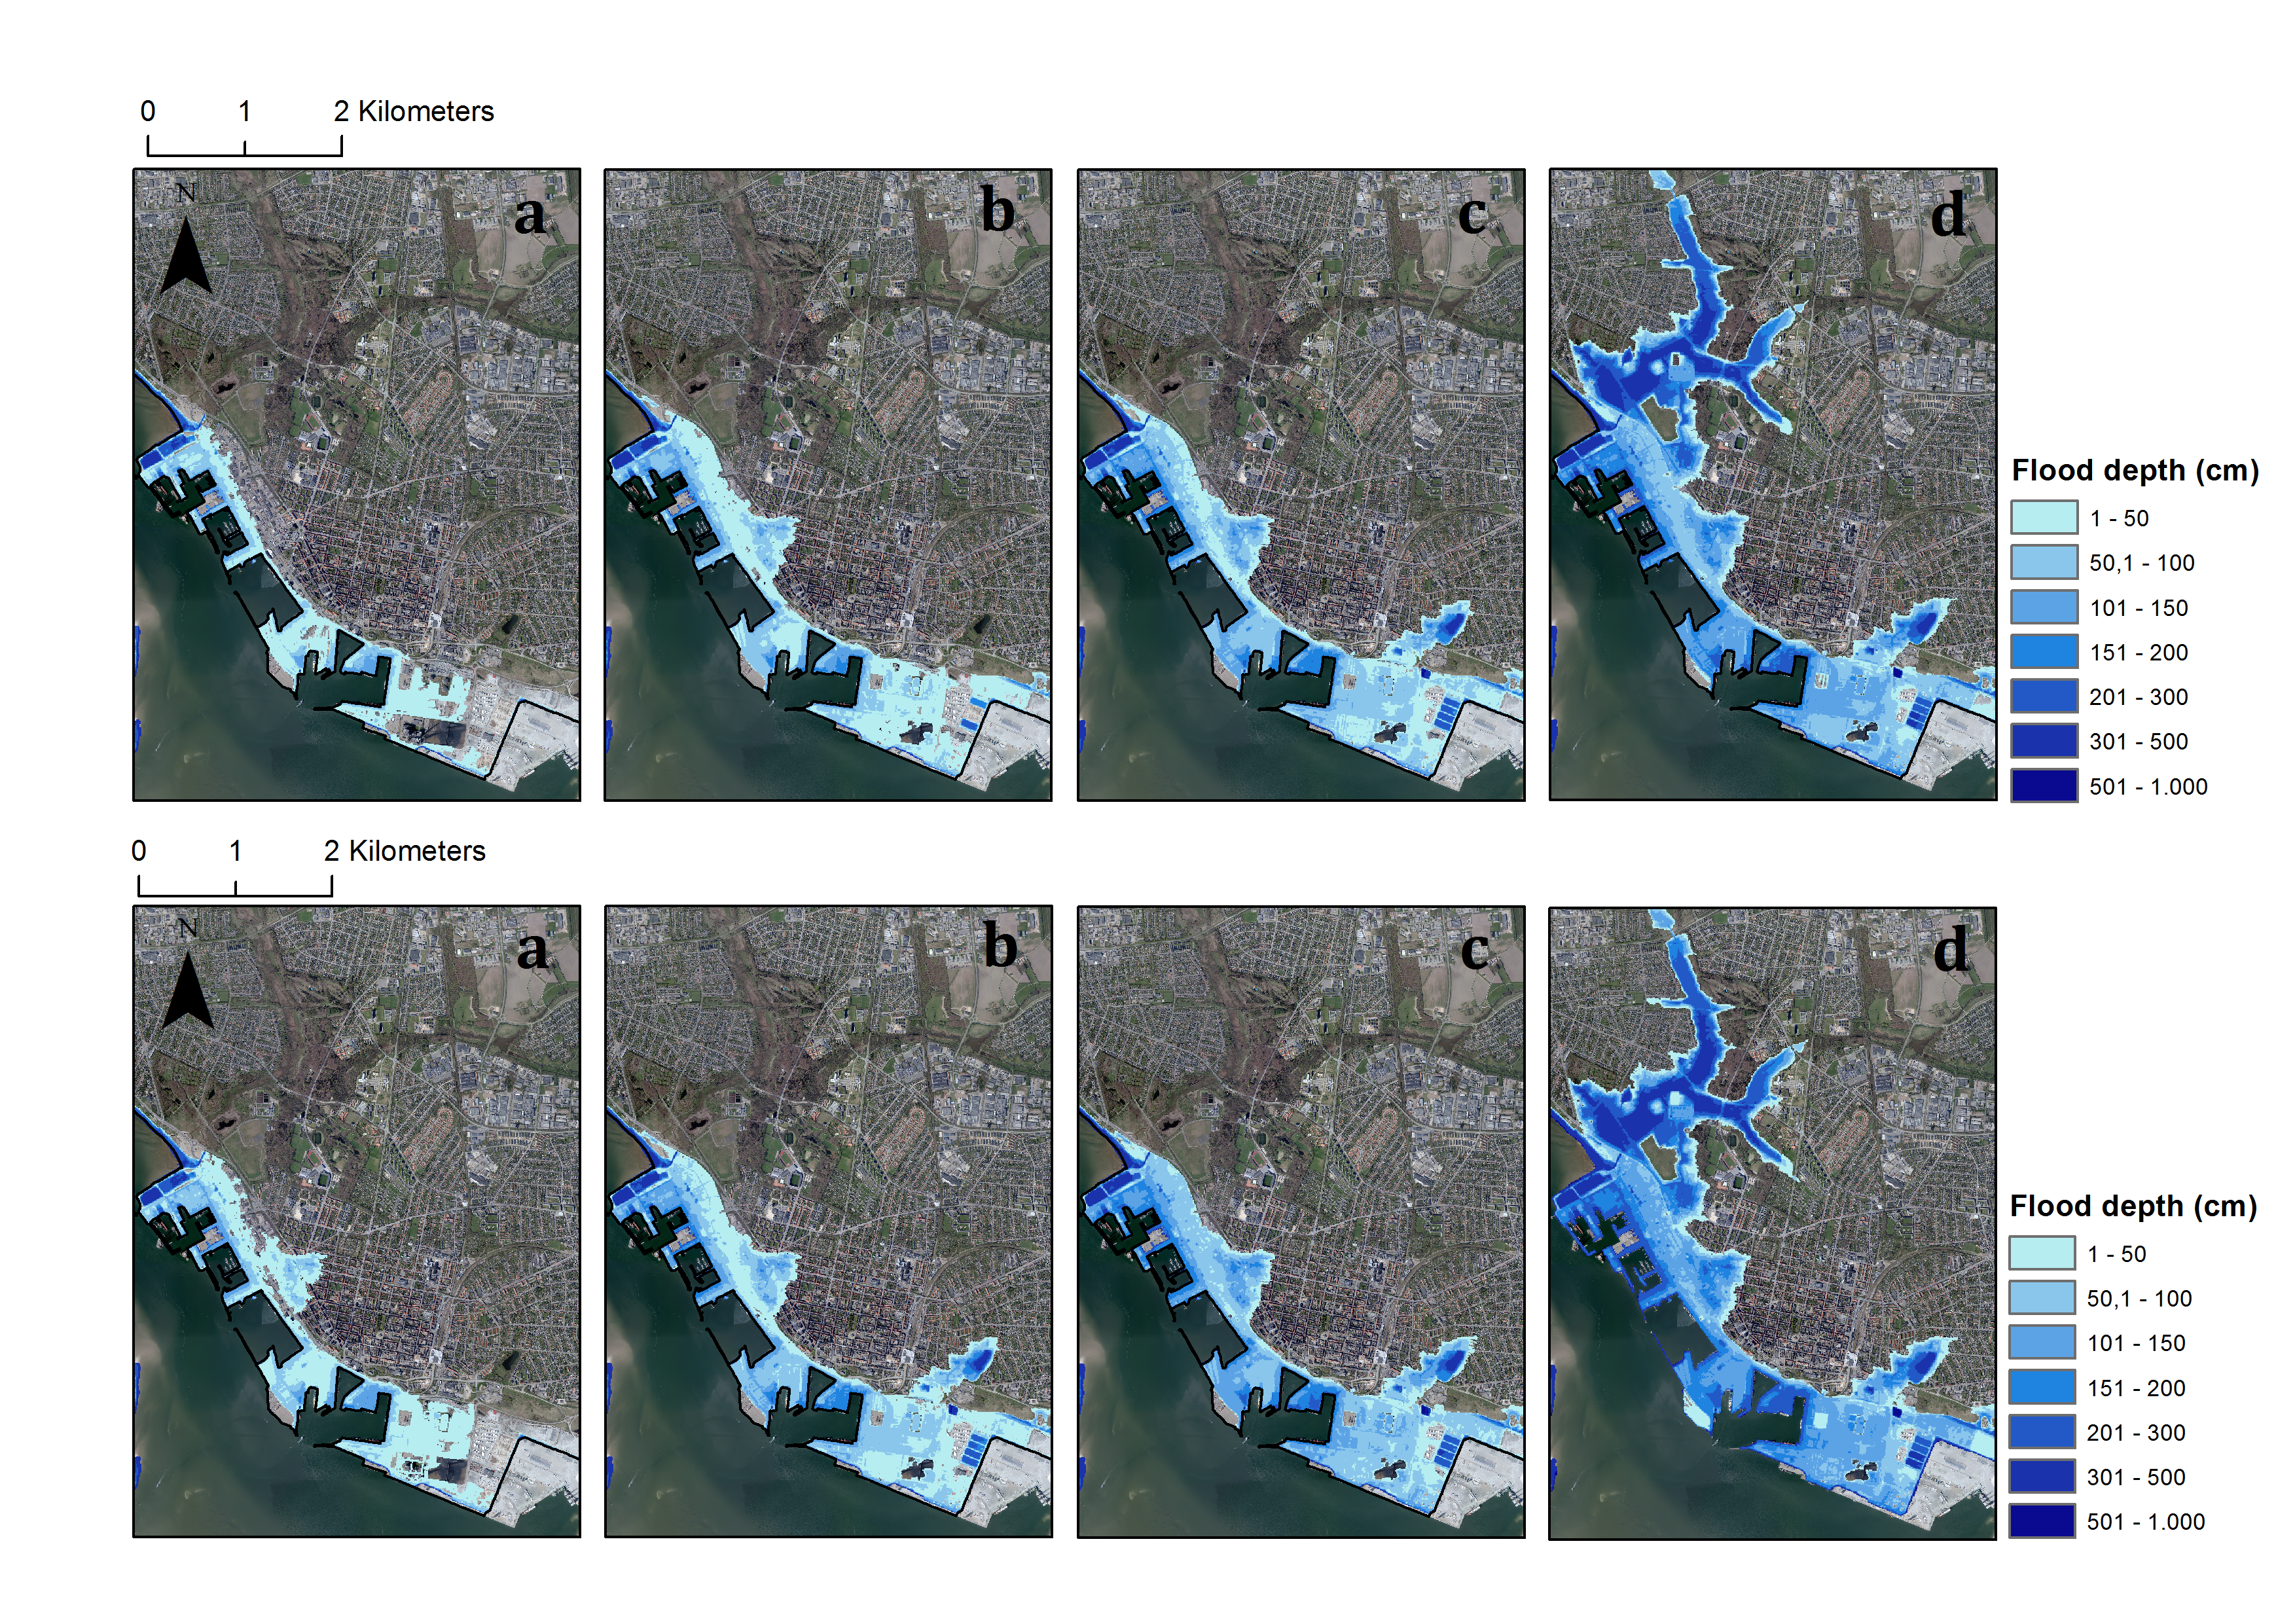
\includegraphics[width=\linewidth]{Floodmaps_Harbour.png}
\caption{Flood extents and depths for the city of Esbjerg in year 2100 during storm surges with a 20 year return period (upper row) and a 100 year return period (lower row) with (a) no sea level rise and with sea level rise corresponding to RCP 85 (5th percentile (b), median (c) and 95th percentile (d)). }
\label{fig:esbjerg}
\end{center}
\end{figure}


\section{The value of including uncertainty}
\label{unc}

\subsection{Sea level projections}

In many cases sea level rise projections are given as a single number for each scenario, usually the mean or median of the ensemble of projections from different climate models (e.g. \citet{climateimpactgroup}). Sometimes the spread of the ensemble is used to assess the uncertainty in the projections (e.g., the Norwegian Environmental Agency recommends using the upper ensemble value for RCP 8.5 as the basis for planning decision, pers. comm. from Even Nilsson, Norwegian Mapping Authority). In our analysis there are two more sources of uncertainty, namely the two regression models. Figure \ref{fig:unc} shows the single number (vertical black line), the ensemble spread (histogram), the uncertainty including only the global model (red) and the full uncertainty (blue) for Bergen projections of sea level rise relative to 1999 under RCP 8.5. We see that the ensemble range is about 16 cm, whereas the overall uncertainty range is about 40 cm.


\begin{figure}[!hbpt]
\begin{center}
\includegraphics[width=0.5\linewidth]{unc.pdf}
\caption{2050 Bergen sea level projections with uncertainty due to different sources for RCP 8.5. The black vertical line is the median projection (with no uncertainty), while the gray histogram corresponds to the spread of the climate models, the red curve adds the uncertainty due to the relation between global temperature and global sea level, and the blue line that due to downscaling global sea level to Bergen. } 
\label{fig:unc}
\end{center}
\end{figure}

\subsection{Damage costs}
A simplistic analysis of projected damage costs at the year 2100, not taking into account the uncertainty, would use  the median  historical damage cost multiplied by  the median damage effect factor at 2100 at the median sea level rise projected for 2100. This yields a damage cost of NOK 338 million (the grey vertical line in Figure \ref{fig:costunc}). Similar results obtain when allowing sea level or effect factor to vary, holding the other quantities at the median (yellow and purple dots on top of Figure \ref{fig:costunc}). However, allowing only the damage cost to vary yields a median cost of 3.85 billion (green dot on top of Figure \ref{fig:costunc}). The appropriate uncertainty analysis for our model should draw each of sea level, effect factor and damage cost at random from their 2100 distributions. This corresponds to a median cost of 3.15 billion NOK, over 9 times higher than the simplistic value. Over 99\% of the costs in our simulation are higher than the simplistic median.

\begin{figure}[!hbpt]
\begin{center}
\includegraphics[width=0.8\linewidth]{UncertaintyLog.pdf}
\caption{Simulated distribution of total damage cost for 2100 without adaptation on log-log scale (black histogram). We also show the distributions of costs varying only one aspect of the uncertainty (sea level rise in blue, effect multiplier in yellow, and damage cost in green), holding the other two at their median values. The grey vertical line is the result of holding all three factors at their median value. The median of each distribution is shown as a dot on top of the figure.} 
\label{fig:costunc}
\end{center}
\end{figure}
\DIFaddbegin 

\subsection{\DIFadd{Risk assessment}}
\DIFadd{The simple spatial analysis carried out for Esbjerg as a screening tool for identifying high-risk areas considers not only the median result but also higher and lower order percentiles as well as different storm surge intensities. Such a probabilistic approach is clearly needed in order to correctly identify areas susceptible to a high risk of flooding, which may subsequently be the subject of more detailed hydrological modelling related to the potential design and implementation of concrete adaptation measures.
}

\DIFadd{Seen from the perspective of a decision-maker, however, adaption actions are likely to be related to an assessment of risk and not hazard. In this study we have not compounded our simple flood risk estimates with the categorical valuation scheme used by Esbjerg in the first phase of their adaptation plan to produce a risk mapping. Hence arguably the design of the original scheme does not discriminate sufficiently between assets to allow for an objective prioritization based on the underlying data, i.e. buildings are generally all assigned a high value, whereas all other assets are assigned significantly lower value. Using a more elaborate valuation model (such a model is currently being developed by Esbjerg municipality in collaboration with consultants) the uncertainties introduced by the valuation model should also be introduced into the probabilistic modelling chain, since the uncertainties introduced by the underlying economic assumptions and modelling (}{\color{blue}\DIFadd{(cite:Halsnaes2015)}}\DIFadd{) may have significant implications on the final results of the risk mapping. One example of this, as already highlighted in the current scheme (Table \ref{tab:valuemap}), is the valuation of natural areas, which in the context of the Esbjerg case in particularly relates to the marshes close to the nearby city of Ribe that are protected under the code of Natura 2000}\footnote{\DIFadd{See }\url{http://ec.europa.eu/environment/nature/natura2000/index_en.htm}\DIFadd{.}}\DIFadd{. From interviews with the municipality it is evident that assigning an objective value to this area, whether by economic cost or in terms of a score, which aligns with the overall objectives of the adaptation plan is a difficult task, which must be taken into account when making the risk assessment including quantification of the uncertainties operational from the end-users' perspectives. 
}\DIFaddend 

%\subsection{...}

\section{Conclusions and discussion}
\label{disc}
Our case studies demonstrate that it is possible to take uncertainty into account in deciding when and where to implement adaptation measures, even if one uses a light touch decision-making approach. If one fails to do so, bad scenarios, such as 95th percentiles, can be a order of magnitude worse than what the planners are expecting. It is likely worthwhile to be pessimistic in the planning and in the projections. 

We consider our case studies proofs of concept, which will be first steps in a sequence of interactions with local planners and other end-users.This has to be an iterative and interactive process, as the decision framework provides actionable information to decision-makers, who will then make their own decisions. These decision can then be incorporated into the current adaptation strategy. Further simulation studies allow a continued loop to identify potential vulnerabilities of the approaches across a wide range of possible futures.

Down the line we plan to develop a flexible and easy-to-use tool kit for decision-making under uncertainty regarding sea level rise. An initial step in this direction is the software used in this analysis, which is publicly available and using free software. 




%  ACKNOWLEDGMENTS
\begin{acknowledgments}
This work was funded by NordForsk through project number 74456 ``Statistical Analysis of Climate Projections'' (eSACP) and The Research Council of Norway through project number 243953 ``Physical and Statistical Analysis of Climate Extremes in Large Datasets'' (ClimateXL). The source code for the analysis is implemented in the statistical programming language {\tt R} (\citet{R}) and is available on GitHub at \url{http://github.com/eSACP/SeaLevelDecisions/Code}.
\end{acknowledgments}

%%  REFERENCE LIST AND TEXT CITATIONS
% 5\bibliographystyle{../BibTeX/agufull08}

\bibliography{ref.bib}
% Please use ONLY \citet and \citep for reference citations.

%\begin{thebibliography}{37}
%%   Before submitting: copy all the contents into the .bbl LaTeX file here
%%   and run latex again
%\providecommand{\natexlab}[1]{#1}
%\expandafter\ifx\csname urlstyle\endcsname\relax
%  \providecommand{\doi}[1]{doi:\discretionary{}{}{}#1}\else
%  \providecommand{\doi}{doi:\discretionary{}{}{}\begingroup
%  \urlstyle{rm}\Url}\fi


%\end{thebibliography}


%% Enter Figures and Tables here:

\end{document}
